%%%% ijcai22.tex

\typeout{IJCAI--22 Instructions for Authors}

% These are the instructions for authors for IJCAI-22.

\documentclass{article}
\pdfpagewidth=8.5in
\pdfpageheight=11in
% The file ijcai22.sty is NOT the same as previous years'
\usepackage{ijcai22}

% Use the postscript times font!
\usepackage{times}
\usepackage{soul}
\usepackage{url}
\usepackage[hidelinks]{hyperref}
\usepackage[utf8]{inputenc}
\usepackage{CJK}
\usepackage{color}
\usepackage[small]{caption}
\usepackage{graphicx}
\usepackage{amsmath}
\usepackage{amsthm}
\usepackage{booktabs}
\usepackage{algorithm}
\usepackage{algorithmic}
\usepackage{multirow}
\urlstyle{same}
\newcommand{\KZ}[1]{\textcolor{blue}{Kenny: #1}}

% the following package is optional:
%\usepackage{latexsym}

% See https://www.overleaf.com/learn/latex/theorems_and_proofs
% for a nice explanation of how to define new theorems, but keep
% in mind that the amsthm package is already included in this
% template and that you must *not* alter the styling.
\newtheorem{example}{Example}
\newtheorem{theorem}{Theorem}

% Following comment is from ijcai97-submit.tex:
% The preparation of these files was supported by Schlumberger Palo Alto
% Research, AT\&T Bell Laboratories, and Morgan Kaufmann Publishers.
% Shirley Jowell, of Morgan Kaufmann Publishers, and Peter F.
% Patel-Schneider, of AT\&T Bell Laboratories collaborated on their
% preparation.

% These instructions can be modified and used in other conferences as long
% as credit to the authors and supporting agencies is retained, this notice
% is not changed, and further modification or reuse is not restricted.
% Neither Shirley Jowell nor Peter F. Patel-Schneider can be listed as
% contacts for providing assistance without their prior permission.

% To use for other conferences, change references to files and the
% conference appropriate and use other authors, contacts, publishers, and
% organizations.
% Also change the deadline and address for returning papers and the length and
% page charge instructions.
% Put where the files are available in the appropriate places.

% PDF Info Is REQUIRED.
% Please **do not** include Title and Author information
\pdfinfo{
/TemplateVersion (IJCAI.2022.0)
}

\title{NoWoC: A Human-AI Collaborative Novel World Creator}

% Multiple author syntax (remove the single-author syntax above and the \iffalse ... \fi here)
% Check the ijcai22-multiauthor.tex file for detailed instructions
\author{
Zhiling Zhang
\and
Kenny Q. Zhu\thanks{The corresponding author}
\affiliations
Shanghai Jiao Tong University
\emails
blmoistawinde@sjtu.edu.cn,
kzhu@cs.sjtu.edu.cn
}

\begin{document}

\maketitle

\begin{abstract}
  This paper presents \texttt{NoWoC}, a human-AI collaborative Novel World Creator leveraging pretrained language models and text-to-image generation models to create a world of story with not only textual content, but also visualizations like character portraits and entity social networks. We also propose theme and entity-description guided generation, which allows users to impose fine-grained control over the generated story with ease. An Integrated Creation Environment (ICE) is designed to support multiple functionalities for the creation and browsing of the heterogenous world. Human evaluation verifies the controllability of the proposed guided generation, and the interestingness of the generated stories. \footnote{Demo video: \url{https://drive.google.com/file/d/13F1Pmw7cfe8IIw9YEN1Nr6rRVfw1CNAO/view?usp=sharing}}
\end{abstract}

\section{Introduction}

Recent progress in controllable generation technique with large models has opened 
up enormous possibilities for human-AI collaborative creativity. They allow users 
to harness the strong generation ability of AI models intuitively using natural language instructions. On the one hand, large pretrained Language Models (LM) like GPT-3 \cite{brown2020language} have exhibited the capability to generate natural and interesting 
story continuations given prime prompts. Later works also explore other natural approaches to integrate human intentions into model generations with various kinds of input as conditions. Examples include story outline \cite{rashkin2020plotmachines}, emotion arc \cite{brahman2020modeling}, game card \cite{akoury2020storium}, intention tag \cite{sun2021iga} and future generation topic \cite{chang2021changing}, etc. On the other hand, Visual-Language Models (VLM) like DALL-E \cite{ramesh2021zero} have demonstrated the capability of creating images from arbitrary text captions for various styles and concepts. The development of user-friendly software or web applications like Story Centaur \cite{swanson2021story}, Wordcraft \cite{coenen2021wordcraft} and AI Dungeon \footnote{\url{https://play.aidungeon.io/}} can further lower the barriers for AI-human collaborative creation and may accelerate the exploration of potentials from these cutting-edge techniques. Better design of effective and intuitive input control, human-computer interaction and exhibition of the outcome remains an open problem to explore.

In this work, we propose Novel World Creator (NoWoC), a human-AI collaborative environment that leveraged large LMs and new controlling strategies to create a holistic world for novel-style texts (see Figure \ref{fig:world_illustration}). The created novel world consists of not only the textual story, but also structural information like entities (e.g. characters, places and other items), their relationships with network visualizations and character portraits with the help of VLMs. 

\begin{figure}[t]
    \centering
    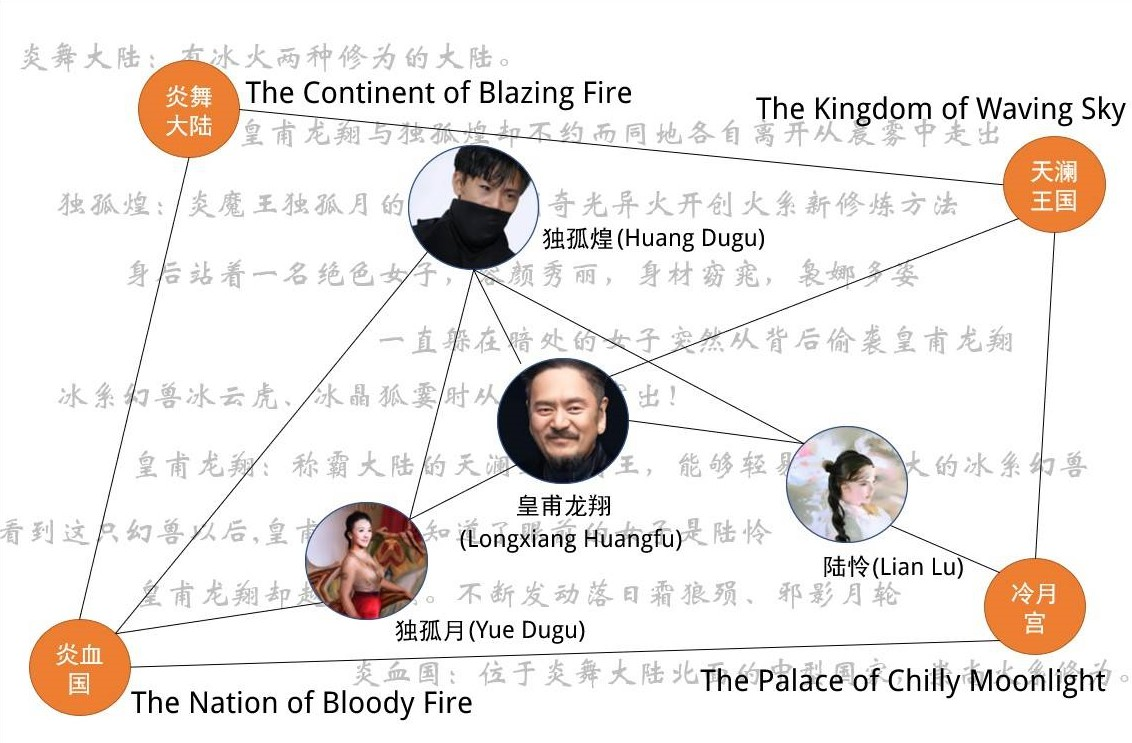
\includegraphics[width=0.98\columnwidth]{figures/english_translation1.jpg}
    \caption{An example novel world from human-AI collaboration. The texts in the background are entities descriptions and story texts. The network reflects the relationship between entities including places (nodes in orange) and characters. The names of the entities and the portraits of the characters are generated by AI.}
    \label{fig:world_illustration}
\end{figure}

To enable the convenient creation of such heterogenous worlds, NoWoC provides a Integrated Creation Environment (ICE) with various generative and browsing functionalities. We also propose two types of user controlled generation strategies: 
theme-guided and entity-description-guided generation. 
Theme is a short phrase for the main topic of generated plot, like war, romance, 
fantasy, etc. 
Entity description can include any information about an entity, 
such as the personality, capabilities and social relations of a person. 
We introduce these strategies to further lower the barrier of creative writing 
so that even users with almost no initial idea on what to write can get a head-start, 
as long as they can come up with entities descriptions from their favorite 
literature works, dramas, movies or even their acquaintances, and pick a theme 
that is likely to produce an meaningful story. Therefore, NoWoC can not only 
help overcome writer's block with its text continuation, 
but also create story beginnings that follow users' anticipated theme 
and entities, which may spark inspirations for further writings.

For the implementation of NoWoC, we resort to large Chinese pretrained models, WuDao 2.0 \cite{dai2019transformer,yuan2021wudaocorpora,ding2021cogview}. We leveraged the strength of these models with carefully designed prompts and in-context learning. We also developed an NLU module to parse information from the generated text and update the world status immediately. Although NoWoC only supports Chinese now, these methodologies can be easily extended to other languages. Therefore, we expect NoWoC to make a general contribution to the design of creative writing systems with human-AI collaboration. 

\section{Functionalities}

In this section, we will describe the various functionalities that NoWoC supports and their implementation methods.

% \subsection{Interactive Generation}
% \label{sec:methods_gen}

% \paragraph{Entity Name Generation} Creating names for entities is often the starting point of writing, and the ability to generate new names has reported to be inspiring \cite{akoury2020storium}. For the generation of character names, we collected a list of Chinese first names and family names, and randomly sample one from each list to combine them into a full name. We generate place names similarly with another lists of common prefixes and postfixes like house, kingdom, continent, etc.

\paragraph{Entity Description Generation} Entity description is the general information about an entity, and will be used to guide the story generation. NoWoC can generate new entity descriptions based on given examples, so that the generated descriptions will resemble the examples and be more likely to cohere with the current world. For example, given fantasy-style character examples emphasizing social status and combat skill, the generated example (in brackets below) will also describe the entity in 
these dimensions. 
% \KZ{English translation for this?}
% \ZL{No space left}

\begin{quote}
    \begin{CJK}{UTF8}{gbsn}
萧炎:本为天才少年,但从十一岁那年开始连续三年莫名其妙地退化成斗之气三段。

药尘:人称药圣,拥有“骨灵冷火”。星陨阁极少露面的阁主,初为九转斗尊巅峰强者。

徐贵:[人称药皇,拥有“大天造化掌”,法尊巅峰。]
    \end{CJK}
\end{quote}

To implement this, we resort to the few-shot in-context learning capability enabled by GPT3-like LM of WuDao. We format the examples as \texttt{\{name\}: \{description\}} one pre line, plus the name of the target entity for creation priming a new line. We then feed the formatted input to the model as the prompt, and let the model complete the 
last line as the description for the new character.

\paragraph{Character Appearance and Portrait Generation} For character entities, we define two extra types of entity information, \textit{appearance} (text) and \textit{portrait} (image).

NoWoC can generate character appearance given the character's gender. The generation is also based on in-context learning, where we collected typical appearance descriptions for each gender, and randomly sample 3 examples of the given gender as input to the backbone model for generation.

Then NoWoC can further generate character portrait given his/her gender and appearance (Figure \ref{fig:portrait}). We initially input \texttt{\{gender\}\{appearance\}} to the DALL-E-like VLM of WuDao for text-to-image generation. However, we notice that the model tends to generate female portraits even if the given gender is male, and it tends to produce non-Chinese characters. To enhance controllability, we replace the \texttt{\{gender\}} in the input with a \textit{reference person}, the name of a celebrity, so that the generated results can inherit his/her prominent features like gender, age and ethnicity. This design also adds fun as users can create their own characters similar to their favorite celebrities. 

\begin{figure}[t]
    \centering
    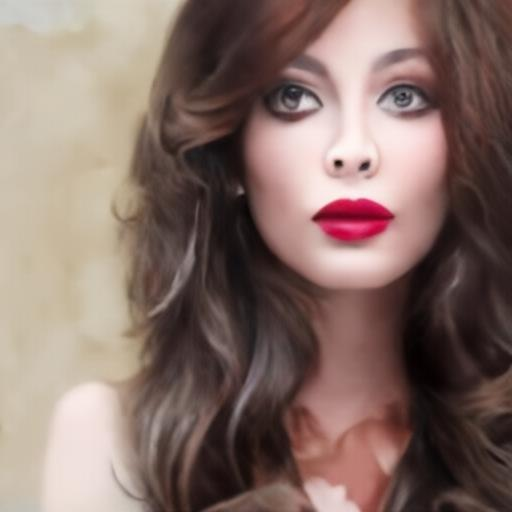
\includegraphics[width=0.48\columnwidth]{figures/gen_3.jpg}
    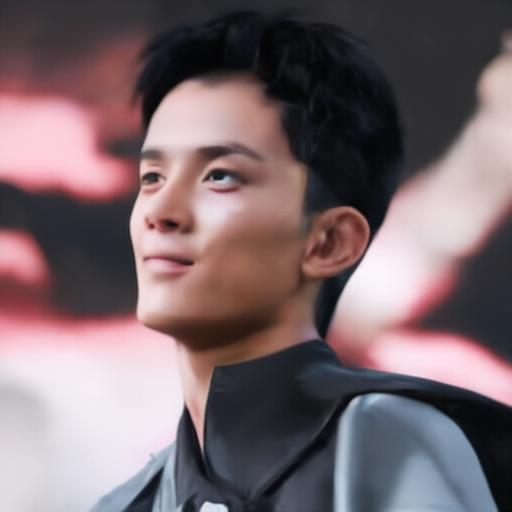
\includegraphics[width=0.48\columnwidth]{figures/gen_1.jpg}
    \caption[caption]{\textbf{Left:} Generated portrait given description: ``He was tall and slender, with lush black hair and peach blossoms-like eyes.'' \textbf{Right:} The generation with additional reference person Leo Wu.}
    \label{fig:portrait}
\end{figure}

\paragraph{Guided Generation} We propose new approaches of intuitive controllable generation, entity description and theme guided generation. First, \textit{entity descriptions} can provide flexible guidance on the generation. For example, if the provided description of the place contains myths about monsters, then the system is more likely to 
generate an encounter with monsters. Next, \textit{themes} can be used specify high-level expectations of the generation. For instance, if we input ``romance'' as the theme, the generated content will be love stories. Moreover, these two types of 
guidance can be mixed. If we provide two characters (A and B) with descriptions about 
their strength (A much stronger than B), and choose a ``fighting'' theme, 
then we may see stories about A defeating B.

To reflect the description guidance naturally in the plot without confusing 
descriptions with stories, we carefully design and test the input prompts 
with several trials. The final prompt format is: 
\begin{quote}
\begin{CJK}{UTF8}{gbsn}
这是一个$\{$theme$\}$的故事$\{$ch\_desc$\}$$\{$pl\_desc$\}$。

一天$\{$period$\}$,在$\{$place$\}$,$\{$character$\}$
\end{CJK}

% This is a $\{$theme$\}$ story$\{$ch\_desc$\}$$\{$pl\_desc$\}$.

% One $\{$period$\}$, at $\{$place$\}$, $\{$character$\}$
\end{quote}
where \{ch\_desc\} is the description of chosen character(s); \{pl\_desc\} is the place description; \{period\} is a time word like morning and afternoon; \{place\} and \{character\} are the names of the place and character(s). The first line includes 
the theme and entity descriptions for guidance, while the second line forms 
a typical beginning of a story, so that story-like texts can be naturally 
generated as the continuation. 

% \paragraph{Continuation} We support generating the continuation of the existing content as a natural application of GPT-like auto-regressive language models. Additionally, we find that the guidance of entity descriptions and theme can also apply here. The guided continuation is achieved with the following prompt: 

% \begin{quote}
%     This is a $\{$theme$\}$ story$\{$ch\_desc$\}$.
    
%     $\{$prev\_content$\}$
% \end{quote}
% where \{prev\_content\} is the previous content to continue writing.

% TODO: If have space, introduce location findings

% \subsection{World Updates}
% \label{sec:methods_update}

% In addition to textual stories, the novel world defined in NoWoC also includes entities and their relationships, which needs to be dynamically updated according to the generation of new content as is discussed above. Entities are stored with structural representation in the system, currently with \textit{name}, \textit{\#occurrence} and \textit{description} (additionally \textit{appearance} and \textit{image} for characters).  A series of NLU procedures are developed to support the following kinds of updates:

\paragraph{New Character/Place Recognition} New entities in the generation that are neither given in the guidance nor defined in the existing world represent
new possibilities to the story and enrich our outlook on the world. 
Therefore, we would like to recognize and register them in our system for later reuse. 
Our definitions of the entity type \textit{character} and \textit{place} are 
largely covered by the common scheme of Named Entity Recognition (NER). 
Therefore, we perform NER on each of the generation, and register new NEs 
with \texttt{Person} type as characters and \texttt{Location} NEs as places.

% \paragraph{New Item Recognition} Items like weapons, treasures and scrolls of secrets can have special functionalities and thus lead to interesting stories. We also want to detect such kinds of items, but most NER system can't recognize them by definition. To tackle this challenge, we draw inspiration from our experience on the typical patterns used in the sentences of their occurrence. Since they are special, the writer usually explicitly states that somebody \textit{discover/find/acquire} them. Therefore, we exploit such pattern by applying Semantic Role Labeling (SRL) on the text. If a sentence has one of the 3 verbs mentioned above as its predicate (\texttt{PRED}), then we will regard its objects (\texttt{ARG1}) as new items. We provide an illustration in Figure \ref{fig:srl}.

% \begin{figure}[h]
%     \centering
%     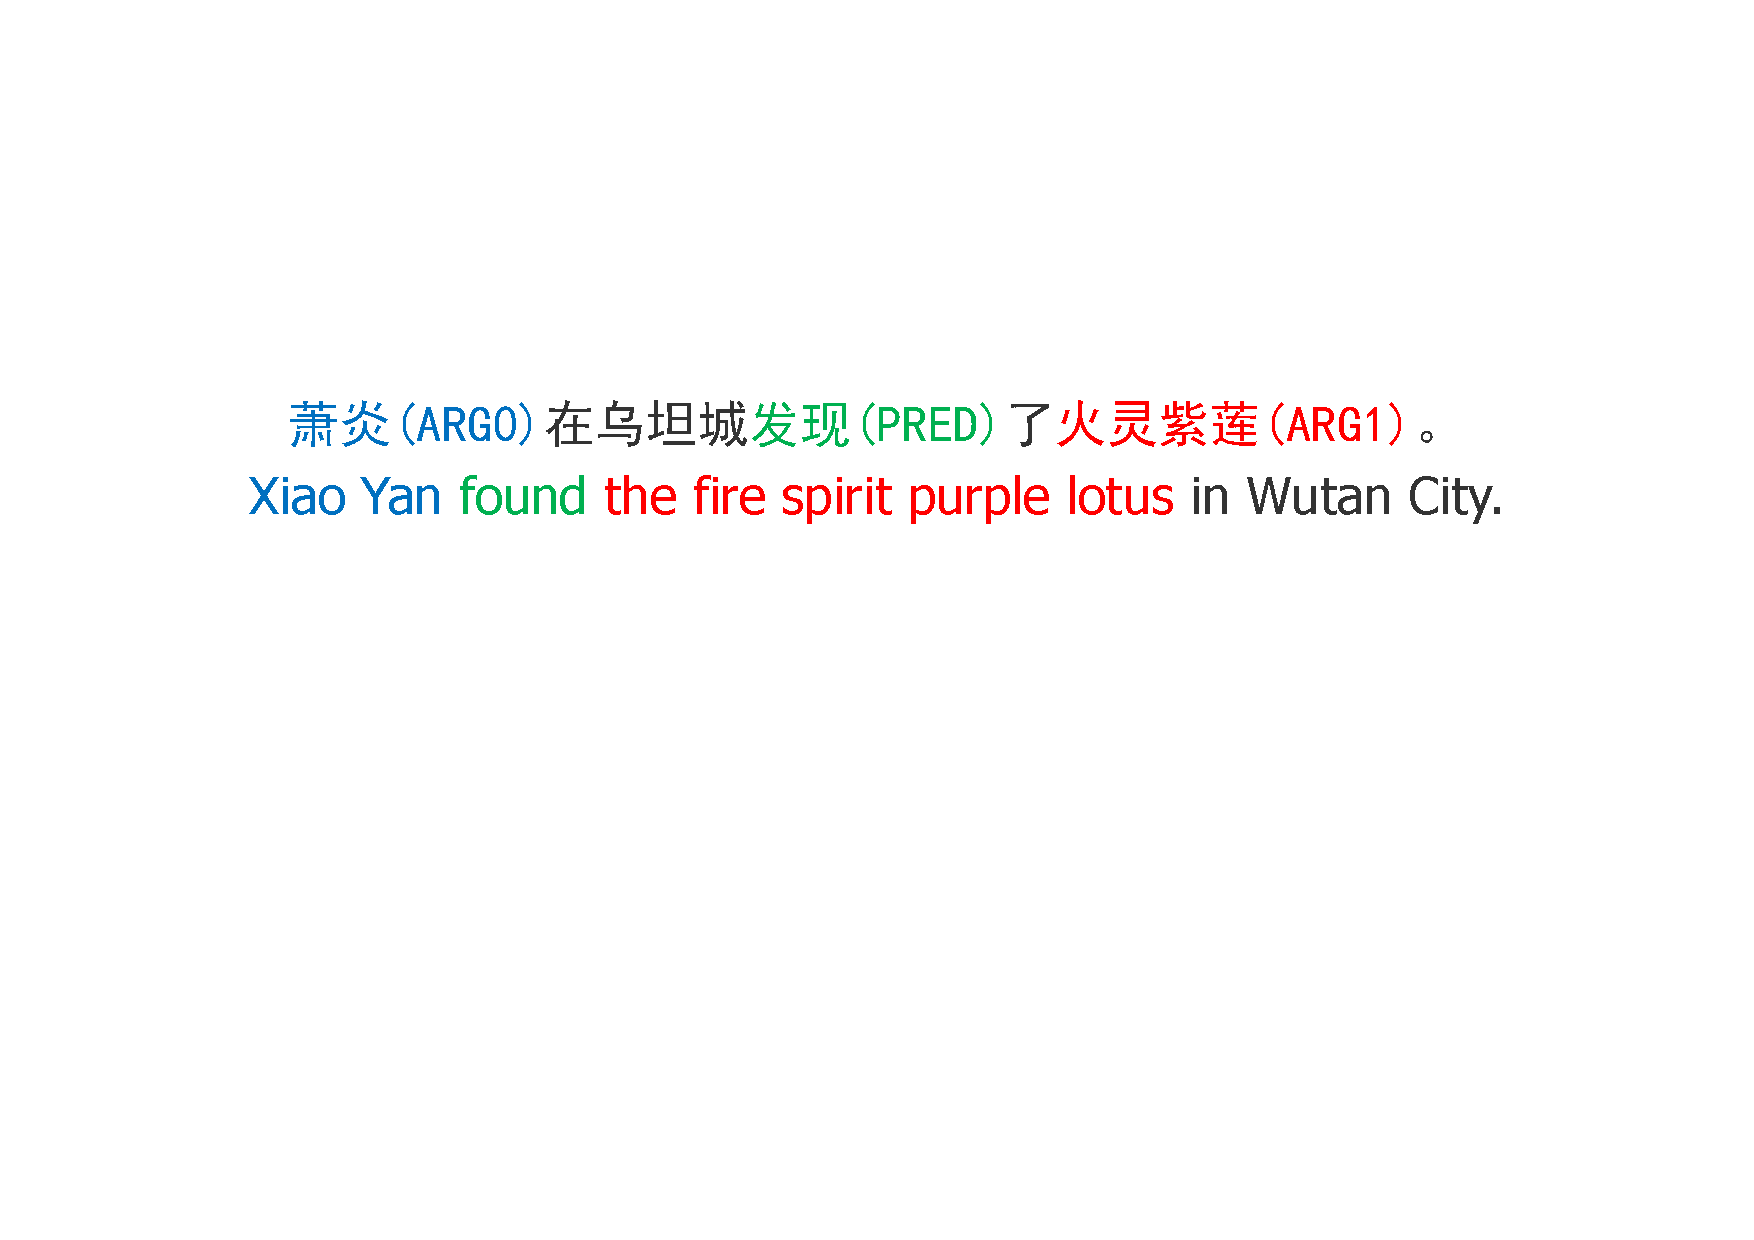
\includegraphics[width=0.95\columnwidth]{figures/srl.pdf}
%     \caption{An example of new item recognition by SRL, where the object ``the fire spirit purple lotus'' will be registered as a new item.}
%     \label{fig:srl}
% \end{figure}

\paragraph{Entity Occurrence and Relation Update} The frequency of occurrence and the relation between entities can help the reader quickly grasp the importance and the positioning of an entity in the novel. NoWoC store entities occurrence and their relations in a weighted graph, with nodes representing entities and edge weights indicating the relation strength. All mentions to the same entities are detected and recorded
in the graph. To characterize relation strength between 2 entities, we rely on 
the hypothesis that the entities co-occurring in near context are likely to be related. Therefore, we add 3 to the edge weight between two entities if they co-occur in 
the same sentence, and add 1 if they co-occur within 2 sentences. 

We omit the discussions on other operations like continuation and entity name 
generation for brevity.

% TODO: If have space, introduce content filtering

% The NER and SRL mentioned above is implemented with a multi-task model provided in the HanLP toolkit \cite{he-choi-2021-stem}, based on ELECTRA \cite{clark2019electra}. Chinese sentence split and entity occurrence detection is achieved with HarvestText \footnote{\url{https://github.com/blmoistawinde/HarvestText}}.


\section{Integrated Creation Environment (ICE)}

\begin{figure}[t]
    \centering
    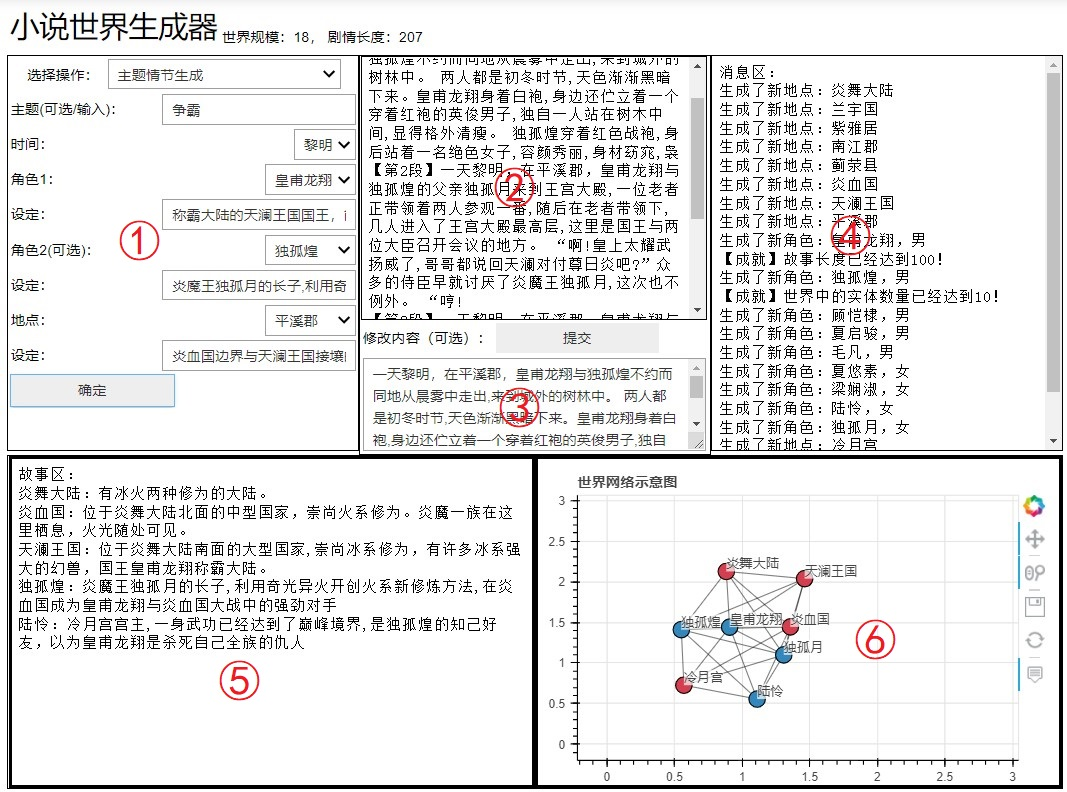
\includegraphics[width=0.95\columnwidth]{figures/environment.jpg}
    \caption{Screenshot of the user interface (numbered parts are 
explained in text)}
    \label{fig:environment}
\end{figure}

To support the creation and exploration of the complex novel world consisting of heterogenous content, we designed a versatile user interface, called ICE. 
The current ICE for NoWoC (Figure \ref{fig:environment}) consists of 5 main parts. 
Part 1 is the main input region, which allows the selection of the operation to 
perform and the input for each operation (e.g., the theme and description for 
guided generation). Part 2 is the output region, where multiple generation results 
from the selected operation will be displayed. User can select their favorite one, 
and polish them in the modification region (Part 3). The multiple choices 
can not only spread the risk of problematic generation \cite{zhang2021diverse}, 
but also provide inspirational examples for users. Similar to the observation 
of \cite{roemmele2021inspiration}, we find that users can learn from the system 
generation to improve their writing. For example, unskilled users can imitate the way model write a story in their own continuation later. % \KZ{How? Any evidence?}  % \ZL{Actually from the user experience of myself. First, I can directly copy content from the choices even not selected (i.e. merge choices given that we can only select one). Moreover, I can also learn from the style of the generated content. }
After the user finished their modification, they can click ``confirm'' and the 
confirmed story content will appear in the story region (Part 5), 
and the notification region (Part 4) will show the new entities recognized from 
the content. Once the user reaches certain goals (like having created more than 
10 entities in the world, or writen more than 100 words in the story), 
we will also congratulate on the user's accomplishment in the notifications. 
Finally, the network of entities and their relations will be dynamically updated and 
visualized in Part 6. The visualization is interactive, so that user can 
zoom in/out to explore certain region of the graph, and check more information of 
an entity by hovering mouse on its corresponding node.

\section{Experiments}

\begin{table}[t]
    \centering
    \small
    \begin{tabular}{lcccc}
    \hline
    Guidance   & C$_{theme}$ (\%) & C$_{desc}$ (\%) & Int$_{[1-3]}$ & Qua$_{[1-3]}$  \\
    \hline
    None       & 25.65             & 16.09            & 1.64                 & 1.34          \\
    Theme-only & 62.28             & 27.64            & 1.94                 & 1.63          \\
    Desc-only  & 60.16             & \textbf{48.25}   & \textbf{1.96}        & \textbf{1.68} \\
    Both       & \textbf{64.1}     & 41.88            & 1.88                 & 1.65         \\
    \hline
    \end{tabular}
    \caption{Human evaluation on generation with different guidance.}
    \label{tab:eval}
\end{table}

Due to the difficulty in making an evaluation of the whole system, we experiment on NoWoC's major component, Guided Generation, instead. We conducted a user study to address two main questions. (1) Are the two types of proposed guidance (theme, entity description) effective in controlling the generation? (2) Can guidance improve the perceived generation quality?

The first author manually wrote 21 story settings (with both theme and entity descriptions). These settings include both adoptions of existing works and new creations. They are designed to cover a wide range of categories (e.g. history, fantasy, romance) and cultures (with both Chinese stories and translated foreign stories) to make a holistic evaluation. 

For each story setting, we generate 6 stories with both guidance (\textit{Both}), single guidance (\textit{Theme-only}, \textit{Desc-only}) and no guidance (\textit{None}). This leads to 4x6x21=504 raw stories. We perform additional post-processing to remove problematic sentences in the stories, and drop stories with less than 30 characters after processing. 469 stories remains.

We invited 4 volunteers to evaluate the quality of the generated stories 
along four dimensions: Conformity to Theme (binary, denoted as C$_{theme}$), 
Conformity to Description (entail/neutral/contraction, with the portion of entailment denoted as C$_{desc}$), Interestingness (scoring from 1 to 3, Int), and 
Quality (1-3, Qua).

Each annotator is randomly assigned half of the stories from each setting, 
so that each story would be rated exactly twice, and we take the average score. % The inter-annotator agreement 
% (according to Fleiss' $\kappa$) for each dimension is 0.39, 0.21, 0.14, 0.06. 
% \KZ{If the kappa is not so big, do u still want to show it?}
% \ZL{If not a big deal, I will hide it. At least we know we have agreement to some extent.}
The results are shown in Table \ref{tab:eval}. It can be seen from the first 
two columns that both guidance, either used separately or together, are effective in controlling theme or description (significantly better than the \textit{None} baseline, $p < 0.001$). They can also significantly improve the interestingness and overall quality of the generation (better than \textit{None}, $p < 0.001$), while the difference between the three kinds of guidance are not significantly different ($p > 0.05$ for each pair). 
% \KZ{Seems desc-only is all you need?}
% \ZL{Possibly, but it may not be bad to have the theme as an additional, valid operation that extends the freedom of user.}

%% The file named.bst is a bibliography style file for BibTeX 0.99c
\bibliographystyle{named}
\bibliography{ijcai22.bib}

\end{document}

